\chapter{Mars Express, MARSIS and ionograms}
In this chapter we introduce the Mars Express spacecraft and its scientific payload. We describe all the appliances, their goals and successes so far. In the second section we present the MARSIS instrument in detail showing the principles of its experiments. The last part of this chapter is devoted to the description of ionograms -- a specific visualization of the ionospheric sounding data from MARSIS. 

\section{Mars Express}
First of all, we briefly introduce the spacecraft carrying all the equipment needed to acquire ionograms. Its name is Mars~Express (MEX) and it was launched by the European Space Agency (ESA) on 2~June~2003. A visualization of the spacecraft is provided in Fig. \ref{fig:mex}.

MEX arrived to Mars at its orbit with periapsis \n[km]{250} and apoapsis over \n[km]{11000} on~25~December~2003~\citep{Chicarro2004} with seven~onboard scientific instruments and a~landing module called Beagle~2. Unfortunately, the landing sequence of Beagle~2 failed (for an unknown reason) and the lander didn't establish connection after it landed (if it landed at all)\citep[p.~4]{Chicarro2004}. 

The mission of MEX has several goals like ``global studies of the surface, subsurface and atmosphere at unprecedented spatial and spectral resolutions'' \citep[p.~viii]{Chicarro2004}. One of the goals, however, stands out among all the others. It is the search for water (or its traces) on martian surface or subsurface.

\begin{figure}
	\centering
	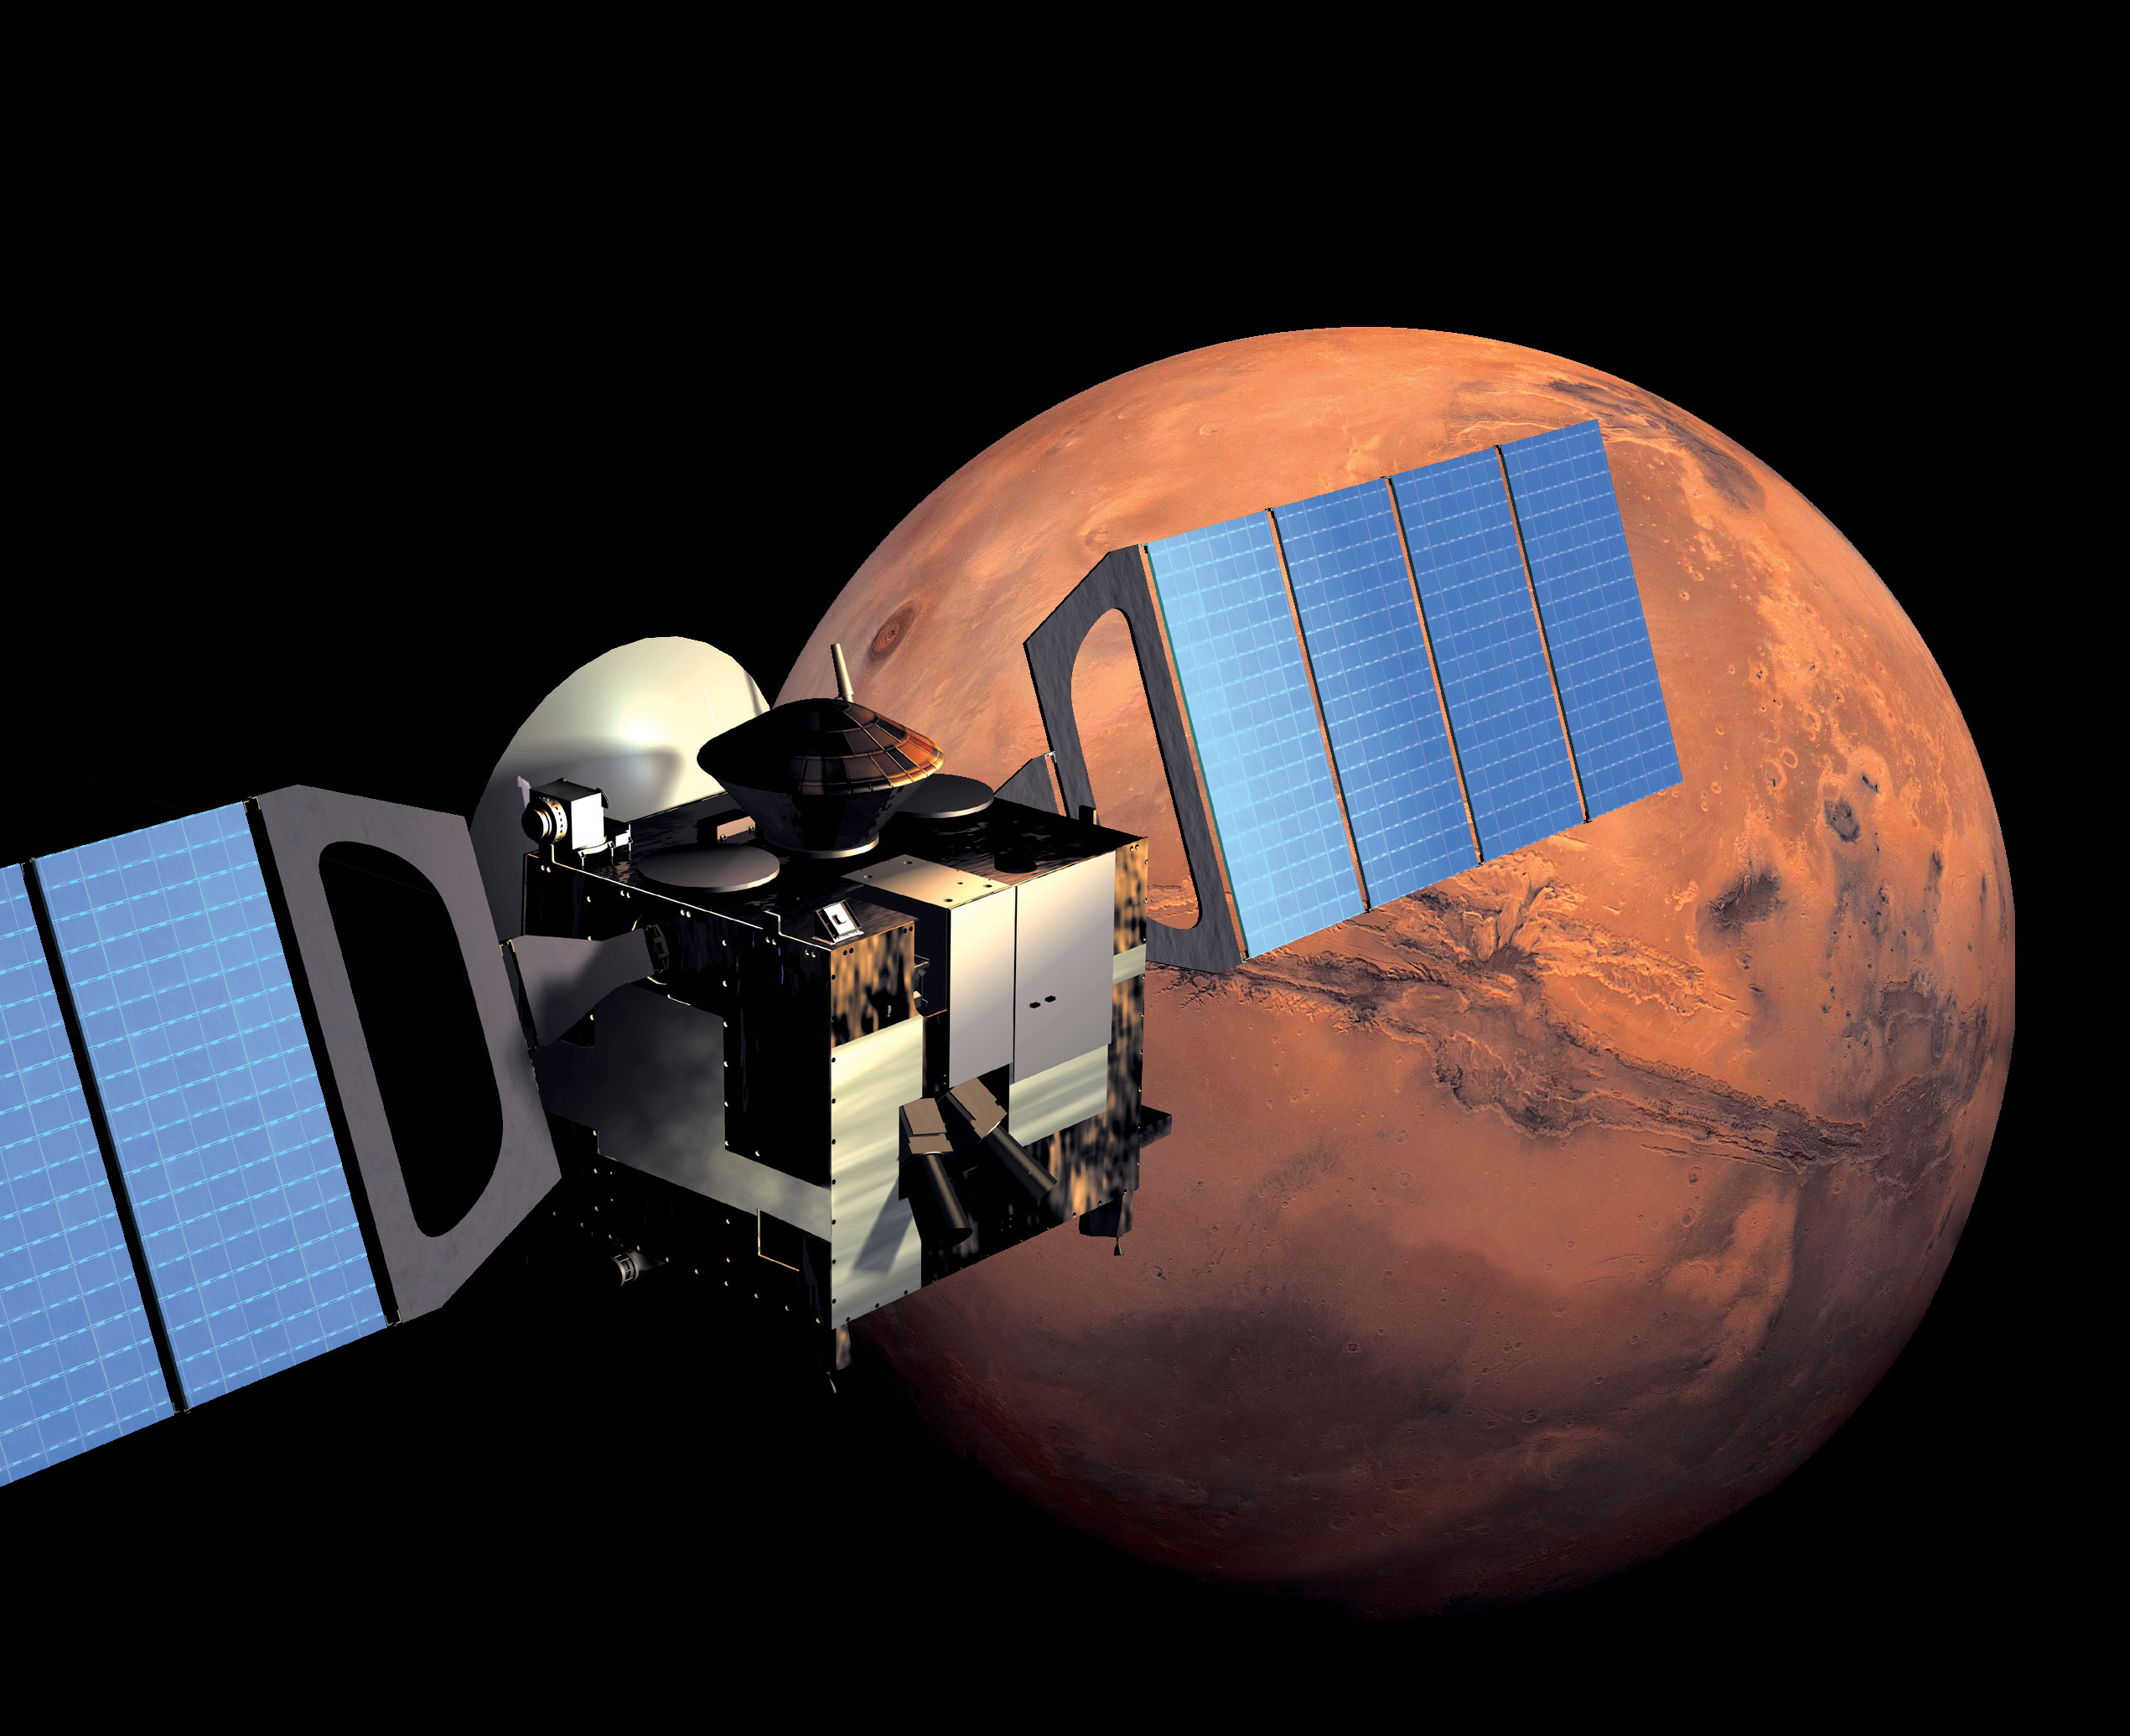
\includegraphics[width=140mm]{images/Mars.jpg}
	\caption{Mars Express spacecraft. \citep{ESA2010}}
	\label{fig:mex}
\end{figure}

There is lots of geological evidence of former water occurrence on~Mars \citep[p.~ix]{Chicarro2004}. But before the~MEX~mission nobody had proved or refuted presence of water on~Mars in the present. Knowing more about water on Mars and its history, the scientists could postulate better hypotheses about the possibility of (former) life on the~planet \citep[p.~ix]{Chicarro2004}. 

The original mission lifetime of MEX was projected up~to the~end of~2005 (which would be 1~Martian~year = 687~Earth~days) \citep{ESA2004}. During its lifetime, MEX encountered some small problems\footnote{as the Solid State Mass Memory anomalies described in~\citep{ESA2011} or the~MARSIS~antennas deployment problems in~2004~\citep{ESA2004a,ESA2005}}. Nevertheless, it has worked on its science goals up to this day and its science mission was extended until~2014~\citep{ESA2013} (after 3~preceding similar extensions). According to Fred Jansen, MEX mission manager, MEX had enough fuel for another 14~years of~operation (at the~beginning of~2012)~\citep{Clark2012}. So there is a hopeful prospect of further and even deeper Mars exploration (e.g. like the~discovery of an~unexpected way of~using the MARSIS~instrument which ``added magnetometer functionality'' to~MARSIS~\citep{Gurnett2005}).

In the~next subsections particular MEX instruments are described. The descriptions are based on~\citep{Chicarro2004} which can be consulted for more detailed information.

\subsection{High-Resolution Stereo Camera (HRSC)}

\begin{figure}
	\centering
	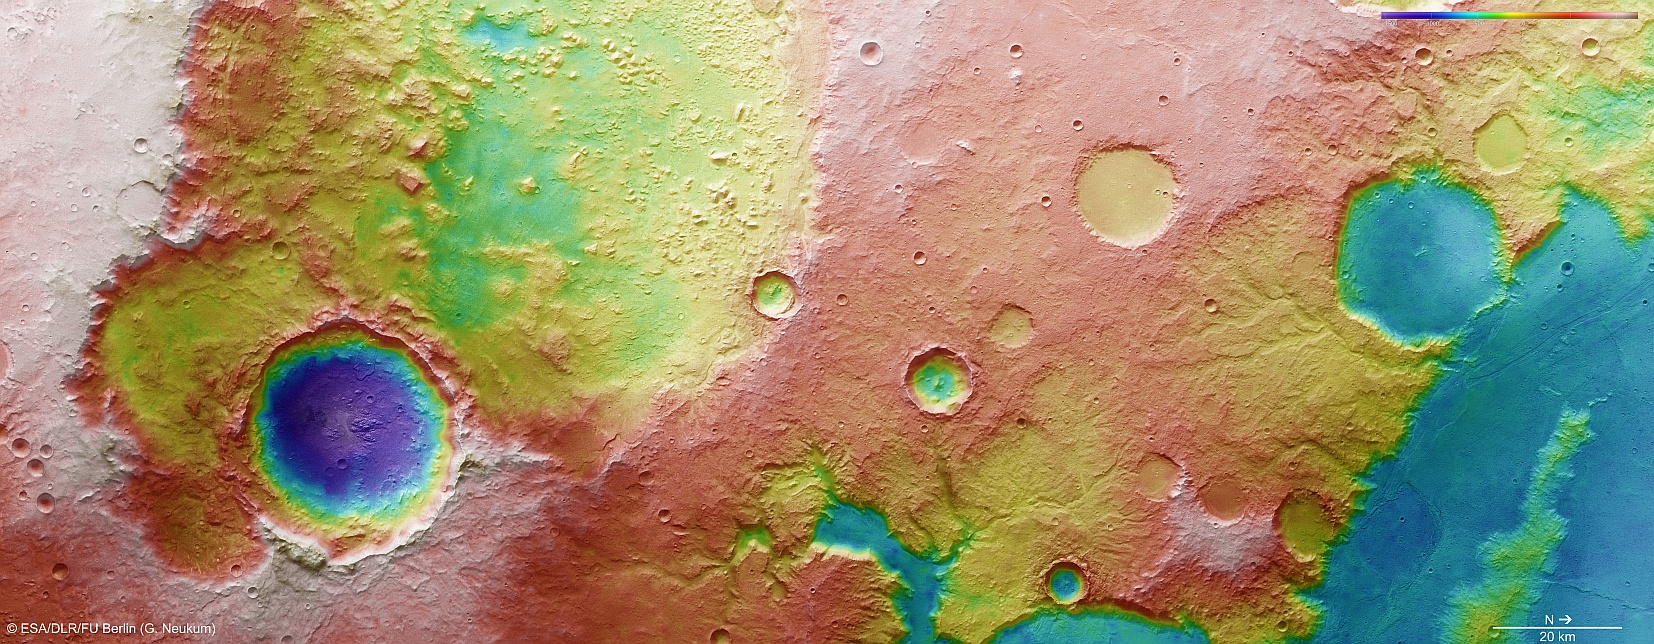
\includegraphics[width=140mm]{images/Topographical_view_of_Amenthes_Planum.jpg}
	\caption{Example image taken by HRSC. \citep{Neukum2013}}
	\label{fig:hrsc_example}
\end{figure}

HRSC is a~high-resolution pushbroom\footnote{A camera that scans the image by rows perpendicular to the flight direction. See \url{http://earthobservatory.nasa.gov/Features/EO1/eo1\_2.php} for more details.} camera for~surface imaging. Its goals are:~\citep[p.~17]{Chicarro2004}
\begin{itemize}
  \item to~characterize surface structure and morphology at~resolution \n[m.px^{-1}]{10} (regions of interest at \n[m.px^{-1}]{2})
  \item to~record surface topology at high vertical resolution
  \item to~observe atmospheric phenomena
  \item to~analyze physical properties of the~surface
  \item to~classify terrain and thus~refine the~martian cartographic base
  \item to~observe martian moons Phobos and Deimos during their approaches
\end{itemize}

HRSC is~able to capture the surface at~resolution up~to~\n[m.px^{-1}]{10} with field of~view~\n[\degree]{11.9}, covering a \n[km]{52.2} wide strip of surface at~height \n[km]{250} (which is the~periapsis of~MEX). The camera consists~of 9~CCD (Charge-coupled device) sensors allowing it to acquire triple stereo images in 4~colors and 5~phase angles. A very useful property of these images is that they are taken nearly simultaneously and thus have the same illumination and other observational conditions (which further helps in photogrammetric processing of the images)~\citep[pp.~24--30]{Chicarro2004}.  

In addition to the stereo camera, the instrument also contains a~super-high-resolution camera called~SRC (Super-Resolution Channel) aimed at~targeted observations of~particular surface details. With image resolution \n[m.px^{-1}]{2.3} and field of view \n[\degree]{0.54} it provides a detailed view of a \n{2.3}x\n[km]{2.35} large surface. Its main purpose is to~take details of~places of~interest, e.g. future landing sites for other landing modules ~\citep[p.~28]{Chicarro2004}.

% achievements
Up to November~2011 HRSC had covered about~\n[\%]{88} of the martian surface \citep[pp.~72--73]{ESA2011a} and still continues to gather new data. An example photograph from HRSC is given in Fig. \ref{fig:hrsc_example}. The scientific results of HRSC are for example:
\begin{itemize}
  \item better exploration of fluviatile valleys \citep{Mangold2008}
  \item discovery of numerous glacial landforms \citep[p.~5]{Fletcher2009}
  \item investigating lava flows \citep[p.~28]{Fletcher2009}
  \item discovery of ``dust devils'' (fast moving dust storms) \citep[p.~47]{Fletcher2009}
  \item providing data to derive a detailed topographic model of more than \n[\%]{20} of Phobos \citep[pp.~945--949]{Jaumann2007}
\end{itemize}

\subsection{Observatoire pour la Min�ralogie, l'Eau, les Glaces et l'Activit� (OMEGA)}
OMEGA is a medium- and high-resolution spectrometer operating in~visible and near-infrared (near-IR) spectra (\n{0.38}--\n[{\upmu}m]{5.1} wavelength). Its medium-resolution operating mode (from heights of~\n{1500} to~\n[km]{4000}) can measure with the resolution~2--\n[km]{5} targeting at global surface coverage. In~the high-resolution~mode (from the~close vicinity of~periapsis) it achieves resolution \n[m]{350} or~better, but can cover only a small fraction of the surface~\citep[p.~37]{Chicarro2004}.

As stated in~\citep[pp.~38--39]{Chicarro2004}, the main goals of OMEGA are:
\begin{itemize}
  \item to~study the~evolution of~Mars
  \item to~detect minerals hidden to~lower resolutions
  \item to~map mineralogical boundaries between geological units
  \item to~reveal gradients in hydration minerals related to~fossil water flows
  \item to~monitor features associated with~wind transportation
\end{itemize}
 
In~particular, OMEGA is intended to find carbonates (not found on martian surface until the launch of MEX) and water ice. It is also able to measure atmospheric pressure, CO and H$_2$O column densities and surface temperature.

Recent contributions of the OMEGA payload are e.g.:
\begin{itemize}
  \item confirmation of liquid water on the surface when the planet was young \citep{Loizeau2012}
  \item discovery of IR and ultraviolet (UV) glows in the atmosphere \citep{Bertaux2012}
  \item proving that Mars had a hot and wet period \citep{Chevrier2007} (implying there were lots of greenhouse gases and a strong magnetic field, too \citep[p.~90]{Fletcher2009})
  \item analyzing the south polar cap and finding out it is formed mainly of water ice \citep{Doute2007}
  \item observation of CO$_2$ ice clouds \citep{Montmessin2007}
  \item finding ferric oxides near the equator \citep{Masse2008}
\end{itemize}

\subsection{Mars Advanced Radar for Subsurface and Ionosphere Sounding (MARSIS)}
\label{ssec:marisIntro}
MARSIS is a long-wavelength radar using coherent wide-band pulses for sounding of the surface, subsurface and ionospehere of Mars. For these purposes it~uses a \n[m]{40} dipole antenna (for both transmitting and receiving) and a~shorter \n[m]{7} monopole antenna (only for~receiving). Due to the used sounding frequencies ranging from \n[kHz]{100} to \n[MHz]{5.5} it is able to reach the depth about 5--\n[km]{8} under the~surface \citep[pp.~51,~57]{Chicarro2004}.

The primary goal of MARSIS is to detect liquid and solid water in the upper crust of Mars. There are also other objectives:~\citep[p.~51]{Chicarro2004}
\begin{itemize}
  \item subsurface geologic probing (to make a~3D characterization of the subsurface structures)
  \item surface characterization (to measure surface roughness, reflectance to radar signals and to estimate topography)
  \item ionosphere sounding (to measure interaction between solar wind and the ionosphere)
\end{itemize}

To name some results of the MARSIS instrument, we can mention the following: 
\begin{itemize}
  \item revealing the layered subsurface structure of both polar caps (strongly suggesting there were oceans in distant history at these places) \citep[pp.~98--102]{Fletcher2009}
  \item estimating the volume of subsurface water ice in the~polar cap \citep{Phillips2008}
  \item discovery of Medusae Fossae Formations (the youngest surface deposits) \citep[pp.~102--105]{Fletcher2009}
  \item mapping the ionosphere and verifying the ionospheric density models \citep[pp.~105-110]{Fletcher2009}
\end{itemize}

One surprising and unexpected utilization of the MARSIS instrument is given by the electron cyclotron echoes found in ionograms (see section \ref{ssec:cyclotronEchoes}). It was found that the echoes often correspond to the strength of the magnetic field, effectively allowing to measure that field and compare it to its model. Another type of echoes, the oblique ionospheric echoes (see section \ref{ssec:oblique}) were identified to correspond to the crustal magnetic field. Both these contributions were made by \citep{Gurnett2005}. 

\subsection{Planetary Fourier Spectrometer (PFS)}
PFS is IR-spectrometer (based on double-pendulum interferometer) operating in the range \n{1.2}--\n[{\upmu}m]{42} divided into two channels -- the Short Wavelength (SW) channel (\n{1.2}--\n[{\upmu}m]{5}) and the Long Wavelength (LW) channel (5--\n[{\upmu}m]{42}). Its spatial resolution is \n[km]{10} for SW and \n[km]{20} for LW (from altitude \n[km]{300}). PFS uses an~onboard Fast Fourier Transform circuit to select only the data scientists are interested in~\citep[pp.~71,~86]{Chicarro2004}.

The objectives of this device are atmospheric studies like:~\citep[pp.~115--116]{Chicarro2004} 
\begin{itemize}
  \item determining atmospheric composition  (as it can detect e.g. H$_2$O, CO and CO$_2$ spectra)
  \item solid-phase surface components detection
  \item atmospheric dust measurements
  \item capturing the vertical temperature--pressure profiles and dust and ice opacity
\end{itemize}

The contributions made using PFS so far are for example:~\citep[pp.~122--135]{Chicarro2004}
\begin{itemize}
  \item measuring the atmospheric temperature (finding out that there is a rather complicated situation around the peak of Olympus Mons)
  \item measuring the surface temperature
  \item counting the atmospheric dust content
  \item observing temperature inversion effects
  \item detecting methane in the atmosphere (which could imply either organic life or volcanic activity, which are both unexpected phenomena)
  \item proving that the south polar cap is made mainly from CO$_2$~ice
  \item capturing the solar spectrum from the surroundings of Mars (which gives results irretrievable from Earth or near Earth)
\end{itemize}

\subsection{SPectroscopy for the Investigation of the Characteristics of the Atmosphere of Mars (SPICAM)}
The SPICAM instrument is made up of two spectrometers, one operating in the UV spectrum (118--\n[nm]{320}) and the other in the near-IR spectrum (\n{1.0}--\n[{\upmu}m]{1.7}). Both these spectra provide information about (not only) H$_2$O in the atmosphere \citep[p.~95]{Chicarro2004}.

Many tasks have been assigned to SPICAM, the major of them being investigating ozone, H$_2$O and aerosols vertical profiles in the atmosphere. These should help with e.g.:~\citep[pp.~97--100]{Chicarro2004}
\begin{itemize}
  \item constructing meteorological and dynamical atmospheric models
  \item understanding the water vapour atmospheric cycles
  \item characterizing processes of water escape from the atmosphere
  \item investigating the interactions between surface and atmosphere
  \item revealing the impact of aerosols on martian climate
\end{itemize}

One of the latest surprises brought by SPICAM is that martian atmosphere is supersaturated with water vapour which further prepares conditions for water escape from the atmosphere \citep{Maltagliati2011}. Another unexpected result are nocturnal aurorae observed in the upper atmosphere, along with the (expected) NO recombination nightglow \citep{Bertaux2005}. Other results involve:
\begin{itemize}
  \item retrieving global spatial and temporal climatology of ozone \citep{Perrier2006}
  \item south polar cap observations \citep[pp.~158--159]{Fletcher2009}
  \item studies of UV dayglow \citep[pp.~160--162]{Fletcher2009}
  \item constructing the aerosol vertical profiles \citep[pp.~175--180]{Fletcher2009}
  \item observation of CO$_2$ clouds on the nightside \citep[p.~178]{Fletcher2009}
\end{itemize}

\subsection{Analyser of Space Plasmas and EneRgetic Atoms (\mbox{ASPERA--3)}}
ASPERA--3 is an instrument designed to study the interaction between solar wind and martian atmosphere. It comprises of four separate detectors. The first detector is Neutral Particle Imager (NPI) measuring the energetic neutral atom (ENA) flux with high angular resolution. Another neutral atoms sensor, the Neutral Particle Detector (NPD), measures the neutral atom flux resolving energy and mass of the atoms. The other two instruments are aimed at electrically charged particles. The Electron Spectrometer (ELS) is a top-hat electrostatic analyzer, while the Ion Mass Analyzer (IMA) is an ion mass composition analyzer working with H$^+$, He$^{2+}$, He$^+$ and O$^+$ ions \citep[p.~122]{Chicarro2004}.

ASPERA--3 should focus on:~\citep[p.~122]{Chicarro2004}
\begin{itemize}
  \item measuring ENAs in order to investigate the interaction between solar wind and martian atmosphere, to characterize the impact of plasma processes on atmospheric evolution and to obtain plasma and neutral gas distribution near Mars
  \item measuring electrons and ions to complement ENA measurements to study the dynamics and structure of plasma and to provide solar wind parameters
\end{itemize}

To present some results of~ASPERA--3 we can mention the following: 
\begin{itemize}
  \item discovering that the solar wind penetrates much deeper in martian atmosphere than was believed, being one of the atmospheric ions escape mechanisms \citep{Barabash2007}
  \item detection of ENA jets caused by solar wind \citep[pp.~208--209]{Fletcher2009}
  \item observing the ENA flux during Mars eclipse which laid foundation of a new method to measure planetary exosphere \citep[p.~209]{Fletcher2009}
  \item proving there is a yet unidentified source of interplanetary ENAs \citep[pp.~209--212]{Fletcher2009}
\end{itemize}

\subsection{Mars Express Orbiter Radio Science (MaRS)}
Opposite to the already described devices, the MaRS experiment does not have a dedicated physical device like a sensor or transmitter. Instead, it utilizes the antennas primarily used for communication to perform radio occultation experiments~\citep[p.~153]{Chicarro2004}. It can use either MEX's parabolic \n[m]{1.6} diameter High Gain Antenna or the smaller Low Gain Antennas attached to MEX. The receivers cannot be carried on board MEX, because they need to be on the opposite side of Mars than MEX is. Thus, the receivers are placed on Earth (Kourou, French Guayana; Darmstadt, Germany; Perth, Australia; three NASA's Deep Space Network telescopes in Goldstone, USA; Madrid, Spain and Canberra, Australia). The experiment uses two frequency bands -- the S-band at \n[GHz]{2.1} and the X-band at \n[GHz]{7.1} \citep[pp.~153--154]{Chicarro2004}.   

MaRS is intended to:~\citep[p.~141]{Chicarro2004}
\begin{itemize}
  \item sound the neutral atmosphere to derive vertical density, pressure and temperature profiles
  \item to sound the ionosphere (in order to get electron density profiles)
  \item to determine the dielectric properties of the surface
  \item to detect gravity anomalies
  \item to sound the solar corona at extra occasions
\end{itemize}

MaRS contributed to e.g.: 
\begin{itemize}
  \item improving existing atmospheric global circulation models \citep[p.~227]{Fletcher2009}
  \item discovering the so-called ``meteor layer'' of atmosphere containing ionized metallic atoms brought into the atmosphere by meteoric impacts \citep[p.~230]{Fletcher2009}
  \item refining the knowledge of structure and density of martian crust~\citep[p.~234]{Fletcher2009}
\end{itemize}

\subsection{Beagle 2}
Beagle~2 is the lander module MEX was equipped with~\citep[p.~165]{Chicarro2004} (its visualization is shown in Fig. \ref{fig:beagle2}). It detached from the spacecraft on 19~December~2003 (6~days before MEX orbit entry) and its touchdown was planned to 25~December~2003. However, it has not transmitted any signal after the martian atmosphere entry. As of February~2004 it was declared lost. No particular reason came out on inquiry into its fault \citep{Bonacina2004}.

To accomplish its main goal (searching for existing or former life, or at least for conditions allowing development of life in the past) it was equipped with the following scientific tools:~\citep[pp.~165--187]{Chicarro2004}
\begin{itemize}
  \item Gas Analysis Package: a mass spectrometer used for examining the surrounding atmospheric gases as well as rock and soil samples (heated in ovens in order to vaporize)
  \item X-Ray Spectrometer: used for studying the composition of rock and soil samples using X-Ray fluorescence spectrometry being able to detect metals like Fe, Mg, Al, Ti and others
  \item M�ssbauer Spectrometer: designed to analyze materials containing iron
  \item Stereo Camera System: intended for acquiring stereoscopic images of the landing site in various spectral ranges
  \item Microscopic Imager: should have provided one of the largest contributions to Beagle's main goal (by searching for microscopic fossils)
  \item Planetary Underground Tool: developed as a support for all the mentioned systems; it should have obtained soil samples using a \n[m]{1.5}~long drill
  \item there is also a grinder available for removing unwanted material from the samples or the surrounding surface
\end{itemize}

There were also several sensors attached to Beagle~2:~\citep[pp.~188--191]{Chicarro2004}
\begin{itemize}
  \item the oxidant sensor monitoring the oxidizing effects of martian atmosphere
  \item the UV sensor capturing the UVA and UVB spectral ranges (which are lethal for organisms)
  \item the wind sensor recording the speed and direction of wind
  \item the air pressure sensor with resolution \n[hPa]{0.003}
  \item the air temperature sensor with accuracy about \n[K]{0.01}
  \item the dust impact monitor measuring the magnitude and impact rate of dust particles
\end{itemize}

\begin{figure}
	\centering
	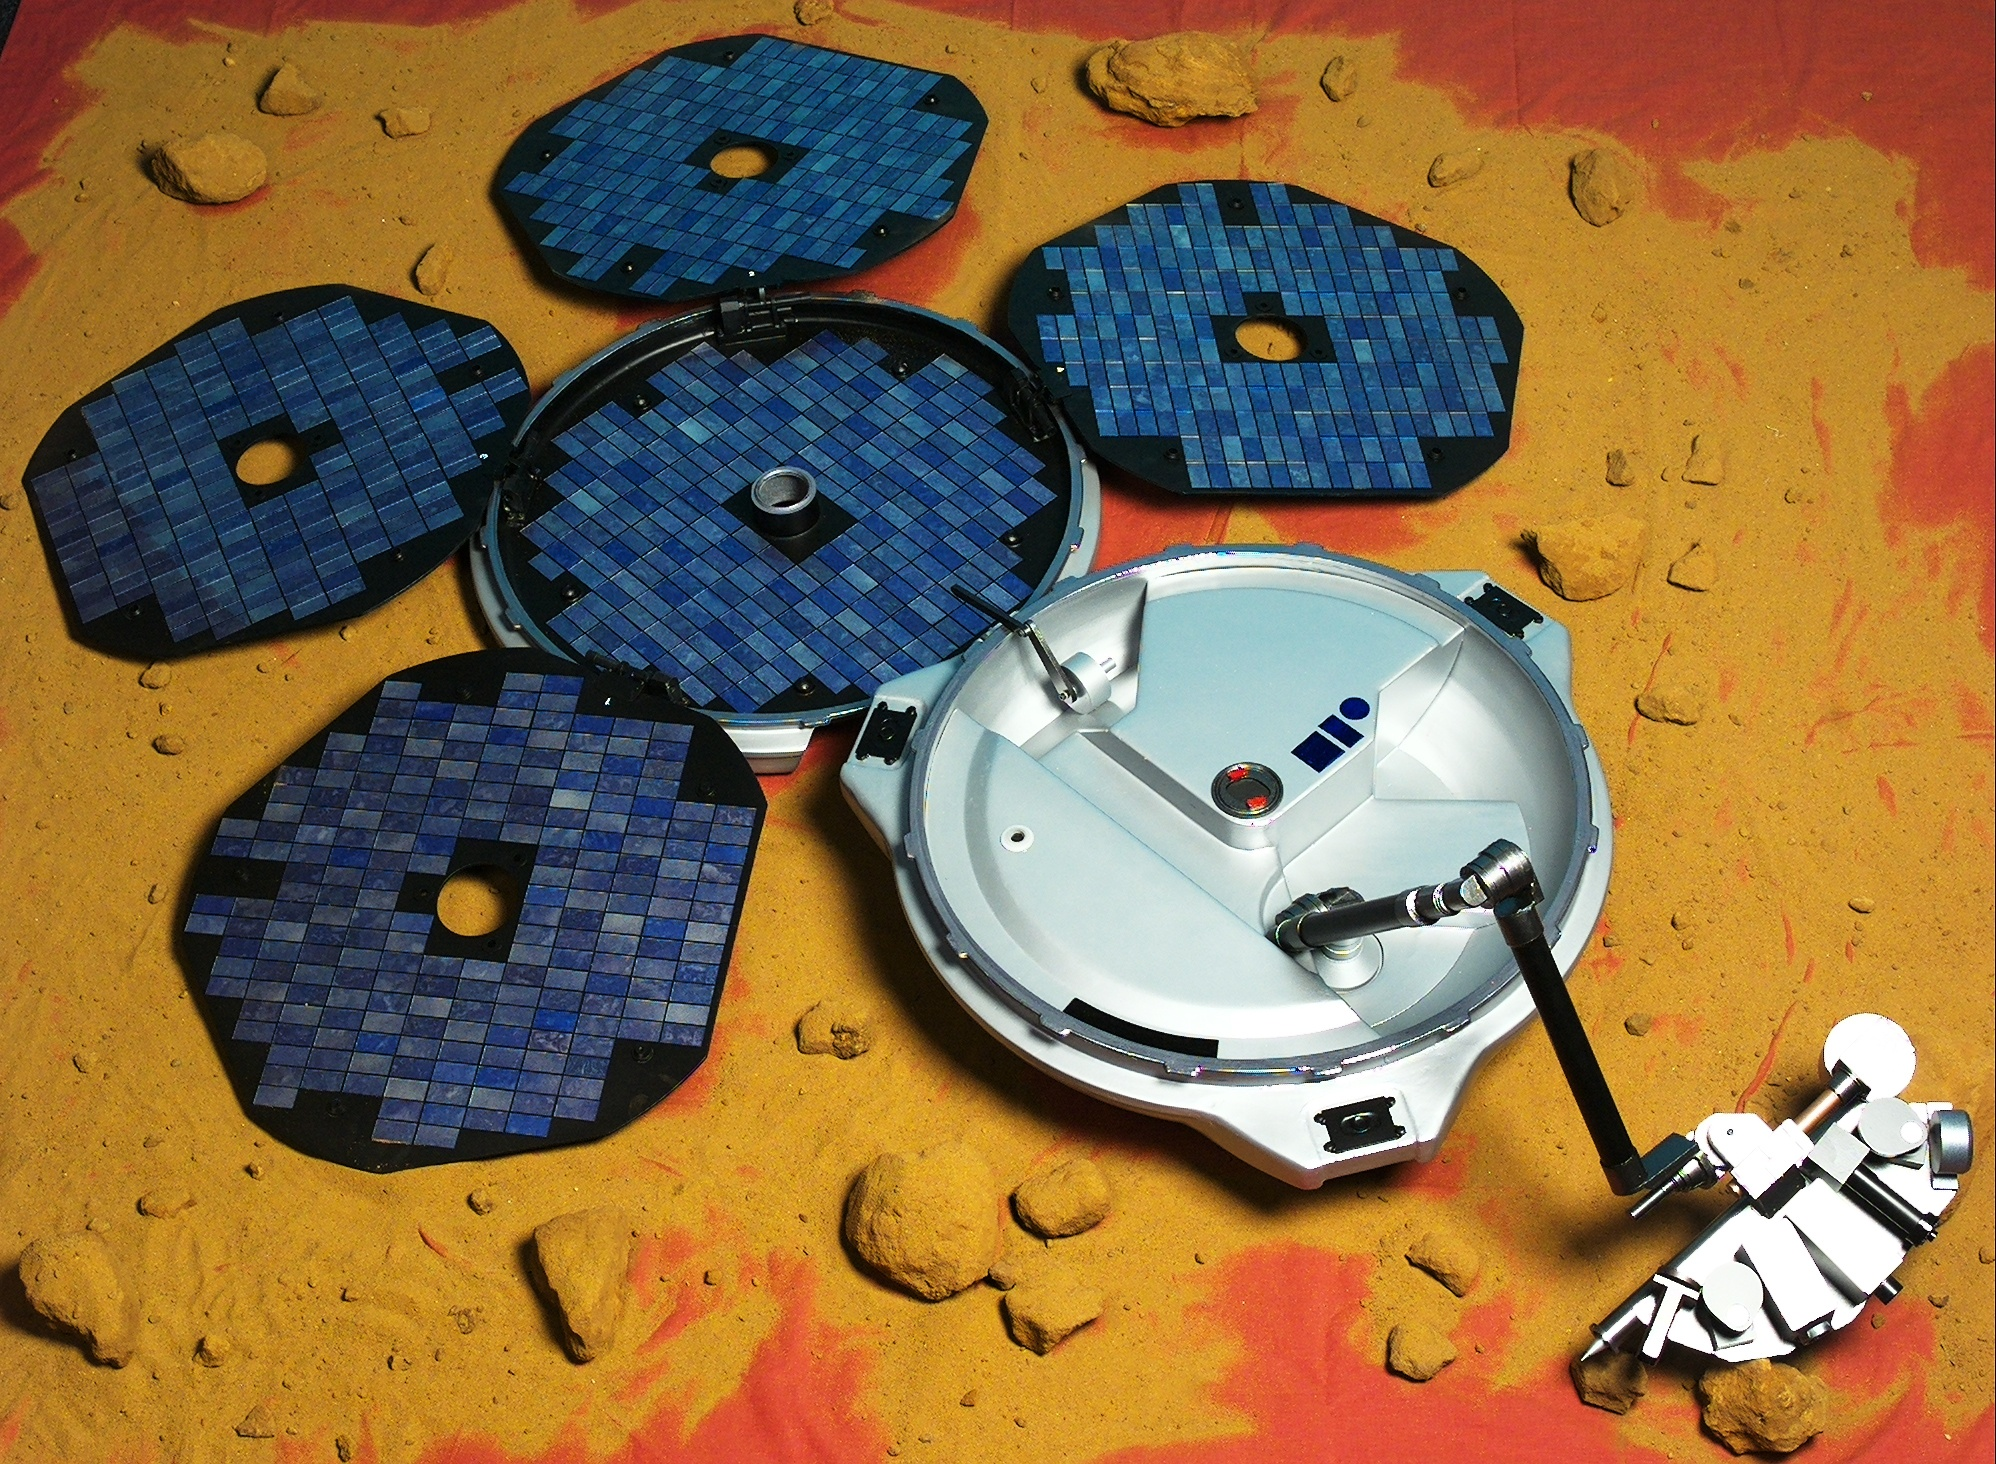
\includegraphics[width=140mm]{images/Beagle_2_lander.jpg}
	\caption{Visualization of the Beagle~2 lander on martian surface. \citep{Beagle2}}
	\label{fig:beagle2}
\end{figure}

\section{The MARSIS experiment}
In this section, we discuss the individual parts of the MARSIS experiment. We briefly describe the physical background of the experiments as well as the technical solution of the measurement mechanisms.

\subsection{Subsurface sounding}
The subsurface sounding attempts to detect the borders of the cryosphere, which is the crust layer in which the temperature remains constantly under the water-freezing point. Such borders can be identified owing to different dielectric properties of liquid water, ice and atmospheric gases. The deeper border can be a water--ice interface. This is because the cryosphere ends at the depth where the internal planetary heat flow raises the temperature above the water-melting point. So if there is a liquid water reservoir under the cryosphere, it can be detected. This interface is expected to be at 0--\n[m]{5000} depth. On the other hand, the higher border can be formed by the desiccated megaregolith (martian soil) where the desiccation is caused by subsurface ice sublimation (estimated to be at depths between 0 and \n[m]{1000}) \citep[pp.~52--53]{Chicarro2004}.

As described in part \ref{ssec:marisIntro}, MARSIS can utilize a \n[m]{40} long dipole antenna as well as a \n[m]{7} monopole one. Only the dipole antenna is used for signal transmission (generating up to \n[W]{10} strong signal), and both antennas for signal receipt. It can sound using one of the four subsurface frequency bands centered at \n{1.8}, \n{3}, \n{4} and \n[MHz]{5}, every one having \n[MHz]{1} bandwidth. When MEX operates on the dayside of Mars, the ionosphere doesn't allow to use lower frequency bands for sounding (see section \ref{ssec:ionospericSounding}), so only the last two bands can be used. On the nightside, all four bands get through the ionosphere and allow to sound deeper subsurface. However, due to the limitations given by the MEX spacecraft, only echoes from depths up to 5--\n[km]{8} can be detected \citep[p.~57]{Chicarro2004}. 

The subsurface sounder mode is based on the fact that the radar waves reflect not only on the surface, but also on subsurface dielectric discontinuities. In addition, the velocity of the waves decreases proportionally to the material loss tangent, the wavelength and the depth -- which facilitates computing the depth of subsurface interfaces \citep[p.~56]{Chicarro2004}.  

\subsection{Surface sounding}
It arises from the previous paragraphs that the surface sounding mode is a ``subset'' of the subsurface sounding mode, taking only the ``topmost'' echoes into account. Therefore, no additional operation modes are present for just the surface sounding. 

The surface sounding is used to create a topography of the surface with lateral resolution 5--\n[km]{9}. This topography further serves for improving the accuracy of statistical topography models which describe the surface in the means of a random distribution of heights \citep[p.~54]{Chicarro2004}.

\subsection{Ionospheric sounding}
\label{ssec:ionospericSounding}
The basic reason for studying the ionosphere is that it stops propagation of electromagnetic waves with frequencies below the local electron plasma frequency $f_p$. This frequency can be expressed as $f_p = 8980 \sqrt{N_e}\mathrm{\ Hz}$, where $N_e$ is the local electron density in cm$^{-3}$. All vertical waves with frequencies below the maximum electron plasma frequency, $f_p$(max), are reflected back at a height with the same frequency as the waves have. This maximum is usually located at the heights 125--\n[km]{150} and amounts up to \n[MHz]{4} on the dayside and \n[kHz]{800} on the nightside \citep[pp.~55--56]{Chicarro2004}.

MARSIS uses two methods -- a passive and an active one. The passive method measures thermal emission at the local electron plasma frequency. The active method -- the one of our interest -- sounds the ionosphere with the radar in 160~frequency steps ranging from \n[kHZ]{100} to \n[MHz]{5.4}. Every pulse has a duration of \n[{\upmu}s]{91.4}. With such a sampling it is possible to construct vertical profiles of the electron plasma frequency (and also electron density). Besides the normal ionospheric sounding mode, MARSIS also provides a special interleaved mode switching periodically between the subsurface sounding and ionosphere sounding modes. This yields a method to remove the ionospheric effects from the subsurface sounding results \citep[p.~58]{Chicarro2004}.

Adding to the ionospheric and surface echoes, there are three more (unexpected \citep[p.~1930]{Gurnett2005}, but useful) signal patterns detectable using the ionospheric sounding. Namely, oblique ionospheric echoes, electron plasma oscillation harmonics and electron cyclotron echoes. We will describe all of them in the following sections after presenting the concept of ionograms.

\section{Ionograms}

\begin{figure}
	\centering
	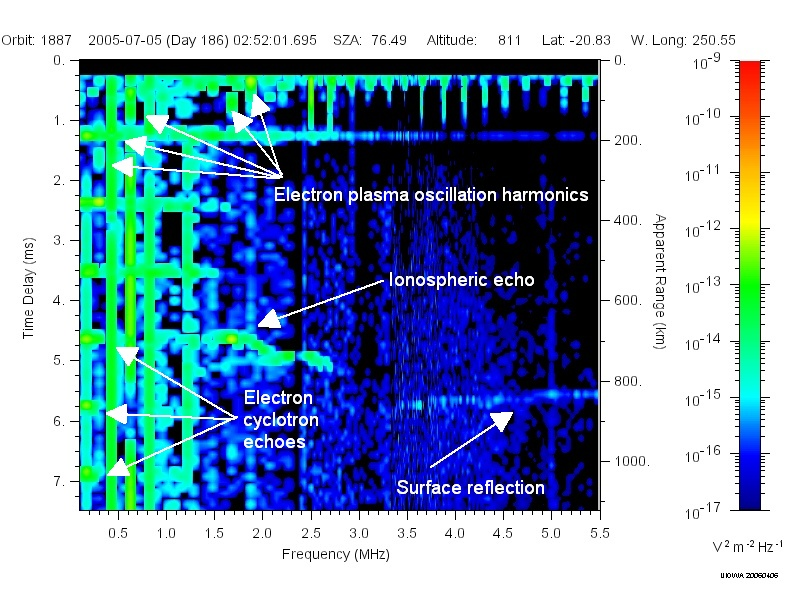
\includegraphics[width=140mm]{images/ionogram_example.jpg}
	\caption{Example of a ionogram showing most of the detectable features like ionospheric echo, surface reflection, electron cyclotron echoes and electron plasma oscillation harmonics. No oblique ionospheric echo is present. The vertical axis shows delay time in ms, the horizontal axis stands for frequency in MHz and color codes the spectral density of the received electric field in V$^2$m$^{-2}$Hz$^{-1}$. Based on real data obtained from \citep{FTP}.}
	\label{fig:example_ionogram}
\end{figure}

Ionograms are the basic visualization of the ionospheric sounding data. Akalin \citep{Akalin2010} defines ionograms in the following precise way:
\begin{quote} 
Ionograms are produced by transmitting a short pulse at a fixed frequency, $f$, and measuring the received intensity at 80~consecutive values of the time delay, ${\Updelta}t$, spaced \n[{\upmu}s]{91.4} apart. The frequency is then incremented and the process is repeated. For each of 160~frequencies, quasi-logarithmically spaced between \n{0.1} and \n[MHz]{5.5}, there are 80~delay time bins, spaced \n[{\upmu}s]{91.4} apart, beginning \n[{\upmu}s]{162.5} after the end of the sounding pulse. Ionograms represent received intensity as a function of time delay and frequency. As shown by the ionogram in Fig. \ref{fig:example_ionogram}, time delay is displayed in milliseconds along the vertical axis, frequency is displayed in megahertz along the horizontal axis, and the color bar represents the received electric field spectral density in V$^2$m$^{-2}$Hz$^{-1}$.
\end{quote}

Several more or less continuous patterns can be found in the example ionogram. Some of them form repetitious patterns. It can be also seen that the data are very noisy. The example ionogram is rather rare, because often just one or two such patterns occur in a single ionogram. There are also ionograms consisting entirely of noise. The subsequent sections will discuss all the patterns and their physical meaning.

\subsection{Ionospheric echo}
As seen in Fig. \ref{fig:example_ionogram}, the ionospheric echo is a horizontally oriented non-straight line. It usually appears in the lower half of the ionogram (delay times about 4 to \n[ms]{5}). Its left end is located where the local f$_p$ frequency starts to be higher than the sounding frequency, which is most often somewhere below \n[MHz]{1}. Its right end should be placed at f$_p$(max) frequency, where all higher-frequency waves pass to the surface \citep[p.~1929]{Gurnett2005}. 

There is often a sharp cusp at the right end of the echo. ``The cusp occurs because the propagation speed of the wave packet (i.e., the group velocity) is very small over an increasingly long path length as the wave frequency approaches f$_p$(max)'' \citep[p.~1929]{Gurnett2005}. On the other hand, the echo often doesn't extend up to f$_p$(max) \citep[p.~1930]{Gurnett2005}.

As we have mentioned earlier, it is possible to read out the local electron plasma frequency from the echo, thus obtaining the electron density vertical profile. In order to extract the profile, it is needed to identify the curve fitting the echo. Automatic identification of such curve is one of the goals of this work. Especially correct estimation of the right end would be helpful if the cusp is present.  

\subsection{Surface echo}
Similar to the ionospheric echo is the surface echo. It is placed lower than the ionospheric echo (because the ionosphere is closer to the sounder than surface is). Its left end is at the same frequency where the ionospheric echo's right end should be, i.e. at the f$_p$(max) frequency. It should extend up to the right edge of the ionogram (since all frequencies higher than f$_p$(max) penetrate the ionosphere) \citep[p.~1929]{Gurnett2005}.

The same (but mirrored) cusp as in ionospheric echo should be present at the left end of the surface echo, caused by the same effect. 

It is common that there is no surface echo in the ionogram. It can have several reasons. One of them is that the surface absorption of the radar waves increases with decreasing solar zenith angle (at angles lower than \n[\degree]{40} the surface echoes are rare). Another way to stop the waves from returning to the sounder could be charged particles from solar flares ionizing the lower levels of ionosphere \citep[p.~1930]{Gurnett2005}.

From surface echoes it is easy to read the apparent height over surface (omitting the cusp area), hence to create topographical maps and models. However, due to the frequent problems with absorption, it is not a good primary means of creating complete topographical maps since lots of the data are missing. 

\subsection{Oblique ionospheric echo}
\label{ssec:oblique}

\begin{figure}
	\centering
	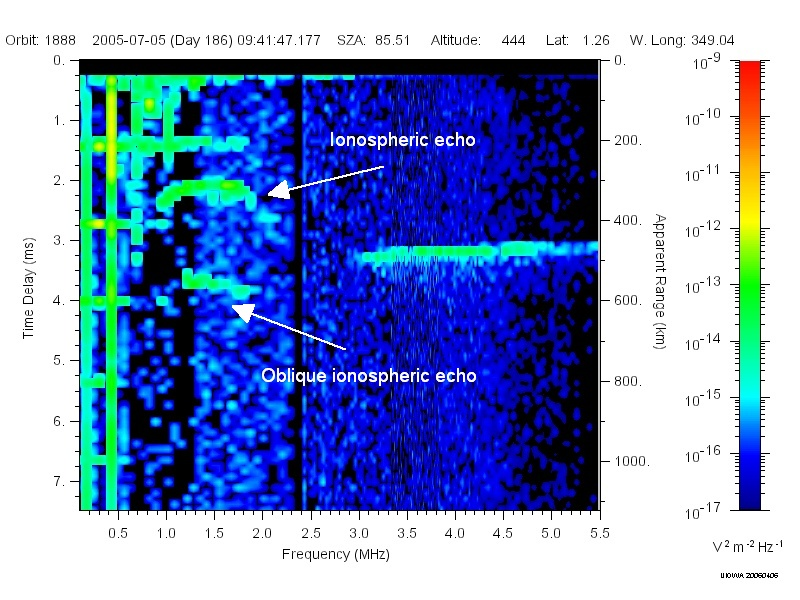
\includegraphics[width=140mm]{images/oblique_echo.jpg}
	\caption{A ionogram containing oblique ionospheric echo. It is worth notice that the echo appears to origin under the surface level (because of the delay time higher than the delay time to surface). Based on real data obtained from \citep{FTP}.}
	\label{fig:oblique_echo}
\end{figure}

The first of unexpected features emergent in ionograms are oblique ionospheric echoes. An example of such echo is displayed in Fig. \ref{fig:oblique_echo}. It is an echo of similar shape and horizontal boundaries as the ionospheric echo, but located a few ms lower in the ionogram. Often even lower than the surface echo -- but the radar waves don't even reach the surface at the frequencies of the ionospheric echo.

\begin{figure}
	\centering
	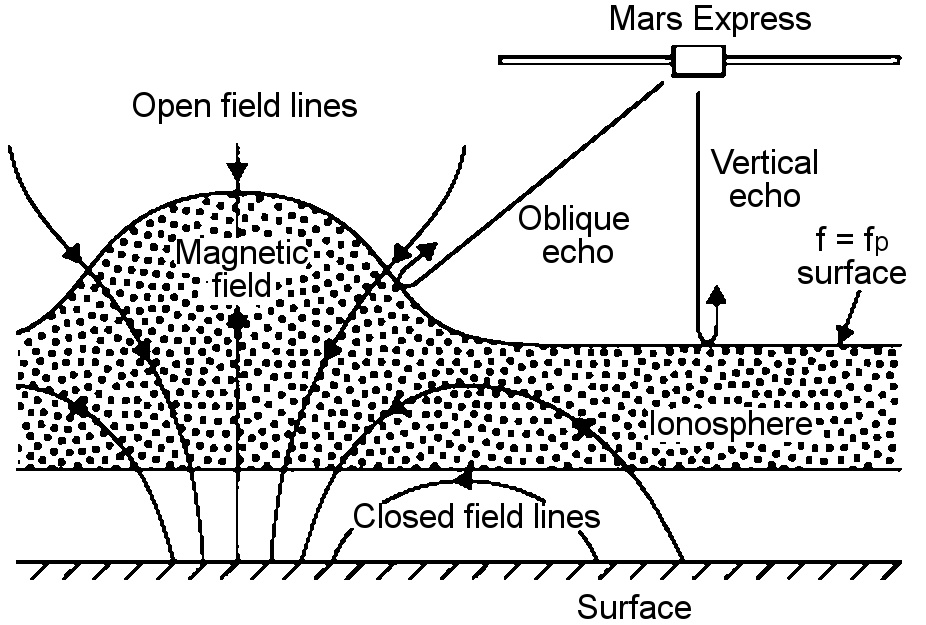
\includegraphics[width=140mm]{images/oblique_explanation.jpg}
	\caption{A ionospheric bulge created by strong crustal magnetic field can produce oblique ionospheric echoes. \citep{Gurnett2005}}
	\label{fig:oblique_explanation}
\end{figure}

An explanation of this effect is given in \citep[pp.~1931--1933]{Gurnett2005}. At locations with strong crustal magnetic field, this field forms bulges in the ionosphere. Such bulges, if lying aside the MEX track, reflect the waves from the sounder under such angle that the antenna records the reflections. However, since the track of these waves isn't vertical, they may travel longer distances than to the surface before they return. An illustration of this effect is provided in Fig. \ref{fig:oblique_explanation}.

To detect oblique echoes in ionograms could be of some use, because they point to places with ionosphere bulges and strong crustal fields. However, deriving the shapes of the bulges or the crustal fields would be very complicated \citep[p.~1932]{Gurnett2005}. Therefore, we won't try to detect them in the task-specific algorithms devised in this thesis. 

\subsection{Electron plasma oscillation harmonics}
Another surprise are repetitious straight vertical lines in ionograms, electron plasma oscillation harmonics (called also Langmuir waves \citep[p.~2]{Duru2008}). As can be seen in Fig. \ref{fig:example_ionogram}, they appear near the top left corner of ionograms. They always start at the top of the image and continue towards the bottom; they may disappear on any time delay. Although they are mainly located in the left part of ionograms, occasionally the may repeat up to the right edge. More than 10~repetitions are, however, rare \citep[p.~4]{Duru2008}.

It is stated in \citep[p.~1929]{Gurnett2005} that these echoes ``are at harmonics of the local electron plasma frequency and are caused by the excitation of electron plasma oscillations, [\ldots]. Even if the fundamental of the plasma frequency is not observed directly [\ldots], the plasma frequency can still be determined from the spacing of the harmonics.'' The reason why not only the base frequency is present, but also its harmonics, is described in \citep[p.~2]{Duru2008}: ``Since the electron plasma oscillations are usually very intense, [\ldots] the received waveforms are often severely clipped. The resulting distortion then introduces harmonics at multiples of the basic oscillation frequency.''

As all features detected by the ionospheric sounder, also plasma oscillation harmonics may not be present in a ionogram. There are three main reasons for it: when the local electron density is less than \n[cm^{-3}]{10}, when the plasma flow velocity is more than \n[km/h]{160} or when the temperature is greater than \n{8521}~$n_e~\degree$K ($n_e$~stands for electron density in cm$^{-3}$; this happens in solar wind) \citep[p.~4]{Duru2008}.

Although the base oscillation frequency is occasionally captured in ionograms (when higher than \n[kHz]{100}, the sounder's lowest frequency), it is apparently more precise to derive the frequency from the harmonics spacing (using multiple fit). That is what we will focus on in later chapters. 

As a benefit, this method allows to measure the electron density in heights up to \n[km]{1300} which corresponds to very low densities. Such low densities couldn't be detected by the radar sounder. 

\subsection{Electron cyclotron echoes}
\label{ssec:cyclotronEchoes}
The last unanticipated phenomenon appearing in ionograms are the electron cyclotron echoes. These are regularly-repeating straight horizontal lines in ionograms. They always start from the lowest sounding frequency (the left edge) and extend to frequencies up to \n[MHz]{2} \citep[p.~3]{Akalin2010}. It can be observed in Fig. \ref{fig:example_ionogram} that the repetition can appear at the whole vertical range.

Comparing with the magnetic field model of Mars, Gurnett \citep{Gurnett2005} determined that the repetition frequency of these echoes corresponds to local electron cyclotron frequency $f_c$. That frequency can be expressed as $f_c~=~28~B~\mathrm{Hz}$, $B$ being the magnetic field strength in nT. Thus, knowing the repetition rate of the echoes, we are able to determine the strength of the magnetic field. That is a very important application, since MEX doesn't carry a magnetometer \citep[p.~1930]{Gurnett2005}. There is also a method to derive the vector component of the magnetic field under some conditions \citep{Akalin2010}.

The origin of these echoes is described in \citep[p.~1930]{Gurnett2005}: ``We believe that these echoes are caused by electrons accelerated by the strong electric fields near the antenna during each cycle of the transmitter waveform. The cyclotron motion of the electrons in the local magnetic field then causes these electrons to periodically return to the vicinity of the antenna, where they induce a signal on the antenna.''

Some constraints, of course, apply to the presence of cyclotron echoes in ionograms. Firstly, the magnetic field strength must be uniform on an area larger than the cyclotron radius (which is about \n[km]{1}). According to \citep[p.~1930]{Gurnett2005} this is easily satisfied. Further, the sounder's minimum and maximum time delay resolution constrains the detectable field strengths. The minimum resolution of \n[{\upmu}s]{182.2} corresponds to field strength of \n[nT]{195}, while the maximum delay of \n[ms]{7.5} corresponds to field strength of about \n[nT]{5}. However, in practice the reasonable range for confident measurements is about 12 -- \n[nT]{160} \citep[p.~3]{Akalin2010}.

Similarly to the plasma oscillation harmonics, we are interested in the period of repetition of these echoes. If we can compute it, we are able to compute the strength of the magnetic field and, in some cases, also its direction. We will also focus on detection of this period in our survey.